\documentclass[10pt]{article}
\usepackage[T1]{fontenc}\usepackage{lmodern,amsmath,amssymb,graphicx,hyperref}
\usepackage[margin=.75in]{geometry}
\setlength{\parindent}{0pt}\setlength{\parskip}{7pt}
\begin{document}
\begin{center}{\Large Positive profiles and integral retained-chart factors}\\[4pt]
Local continuation --- 16 November 2026\end{center}
Let $t$ be an actual nonzero retained integer grid node with valuation
$i<u\le a$, and put $q_i=\min\{2,u-i-1\}$. For the same common profile
$m=4n$, the existing full odd-right content bound permits the actual
rational-polynomial rescaling
\[
 L'_{x,(r,b)}=2^{g_b}L_{x,(r,b)},\quad
 R'_{(r,b),y}=2^{-g_b}R_{(r,b),y},\qquad
 g_b=\begin{cases}q_i&b\text{ odd},\\0&b\text{ even}.\end{cases}
\]
The exact product $L'R'=LR$ and original full residual are preserved.
Right entries are integral. Left entries have content at least
$w+b+g_b$, and are integral when $w\ge0$ [pcc:unverified].

\textbf{Product law.} The rescaling is inserted as mutually inverse
bundled diagonal units in $\mathbb Q[Z]$. Existing rectangular Matrix
laws give the product identity. These are not units in the two-integral
coefficient ring or in characteristic $2^p$. Integrality is derived
separately from the actual full content theorem. No inverse of two in a
finite ring is introduced [pcc:unverified].

\textbf{The profile is constructed.} On $\operatorname{Fin}(u)$ set
\[
 U_{ij}=(j-i)_+,\qquad S=\sum_{r<u}U^r,\qquad n=S\mathbf1.
\]
Extend $n$ by zero outside the finite domain. Strict upper triangularity,
the existing characteristic-polynomial formula and Cayley--Hamilton give
$U^u=0$; the natural-coefficient case follows by the existing injective
map to integers. Existing semiring geometric identities yield
$n=Un+\mathbf1$. Hence each retained $n_i>0$ and the original schedule is
\[
 G_i(n)=n_i-\sum_{j<u}(j-i)_+n_j=1,\qquad G_i(4n)=4.
\]
This supplies the required nonnegative left weight at $i<u\le a$,
without a caller-supplied favorable schedule witness [pcc:unverified].

\textbf{The mass is charged.} The exact total mass quadruples under
$m=4n$. At $u+1$ retained levels, the existing actual budget theorem gives
\[
 \sum_{j=0}^{u}m_j\;\ge\;4F_{2u+1}.
\]
This is a necessary mass for this profile family. It supplies neither a
low global degree cap nor an algorithmic lower bound [pcc:unverified].
\newpage
\begin{center}{\Large Evidence and the next cost bridge}\end{center}
\begin{center}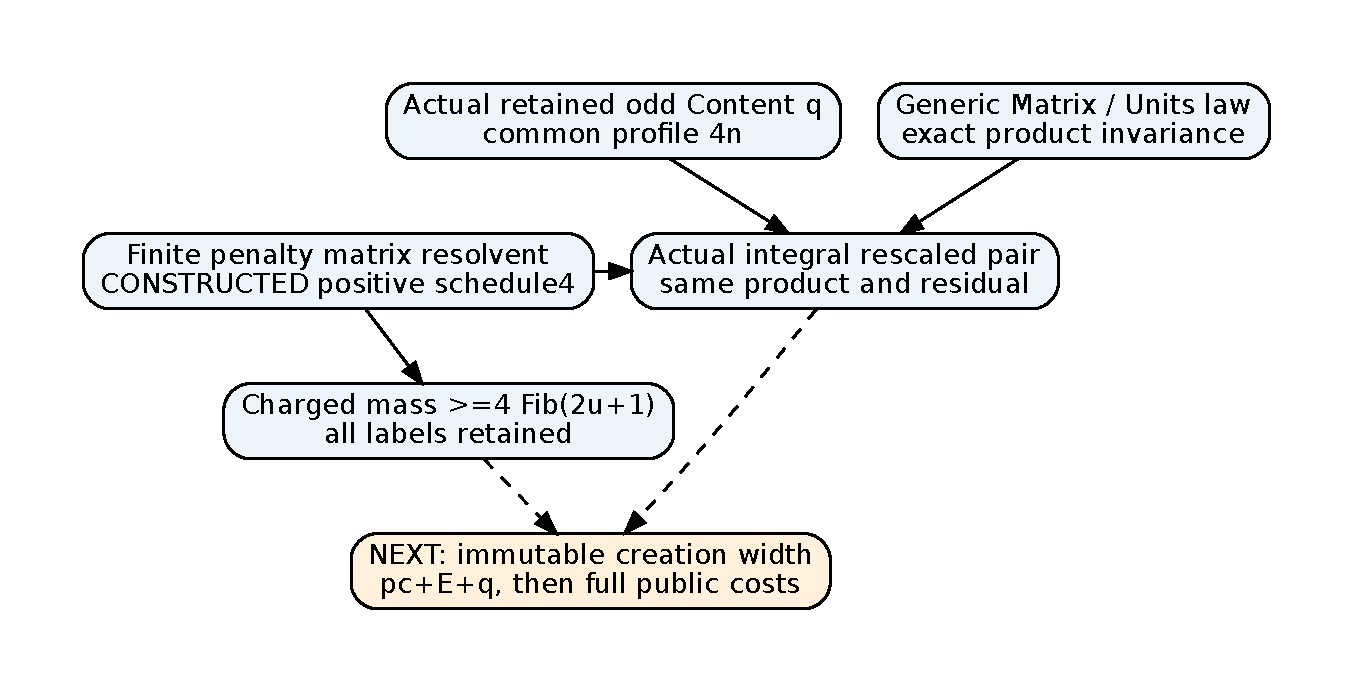
\includegraphics[width=\linewidth,height=2.25in,keepaspectratio]{rescaling-profile-dependencies-001.pdf}\end{center}
\textbf{Local evidence.} Study112 compiles472 named source statements
including historical458, with14 new actual rescaling instance contracts.
Standalone profile114 has11 actual construction statements. Combined115
has485 including458, with27 new instance and semantic contracts;
all three exit zero without warnings or sorryAx. Central printed
axiom dependencies are standard. Receipts060,062 and063 bind the exact
sources, raw outputs and exits [pcc:unverified].

\textbf{Owning-library laws.} CryptoLean commit8ae174d composes one generic
rectangular unit-rescaling law from existing Matrix and Units laws;
commit2fc4da5 adds three strict-triangle and nilpotent-resolvent laws.
The existing pinned module auditor reports respectively one and three
theorems, zero failing and zero trusted. These scoped audits do not cover
every study statement. All new records are unsigned and defaultnot\_covered;
the study is outside shared Transport53/57/fresh coverage. The consumer
manifest is unchanged; the experimental owner overlay is explicit
[pcc:unverified].

\textbf{Failures retained.} Study108--110 failed private-definition and
matrix instance elaboration. Small probe111 established the exact chained
entry law used by112. Owner strict-triangle001--003 failed cast and map
API elaboration;004 passes. Profile113 retained a deprecated-name warning;
114 uses the current name. Every failed source, raw output, exit and
pre-call hash is preserved. No linter, opacity or trust waiver was used
[pcc:unverified].

\textbf{Next obligation.} A divided right entry at creation precision
$p_c$ requires numerator information at width $p_c+E+q_i$, with the
\emph{same} creation truncation and labels; $E$ is the old denominator's
valuation. The denominator becomes $D2^{q_i}$. Division of an old
$p_c$-bit representative does not supply the missing digits. Protocol018
requires canonical reduction, signed and zero cases, then immutable
freezing, and charges all extra preparation and extraction work
[pcc:unverified].

Every $2^u k$ label remains charged. Actual nonzero mode inventory, child
interfaces, degree and recursion, representation preparation and full
public expected bit cost remain open. Same auxiliary $W$ and origin;
no jet-completion $H$ or nonscalar origin has been selected. No native,
paid, timing, scaling or attack campaign was run. Publication remains
local under the protected remote ledger conflict [pcc:unverified].
\end{document}
